%% PRESENTATION MODE
\documentclass[
    utf8,
    aspectratio=169
]{beamer}  % We could consider beamerswitch.
%% ARTICLE MODE
%\documentclass[utf8]{article} \usepackage{beamerarticle}

%%% 1. Praeambulum
% Siehe http://www.staff.uni-giessen.de/partosch/unterlagen/Abschlussarbeit-Anleitung.pdf
\usepackage[english]{babel}
\usepackage[%
	backend=biber, %biber would be better, but doesn't work for me so far
	%backend=bibtex8,  %use this backend if biber does not work
	%style=authoryear
	style=numeric,
	maxbibnames=99
	]{biblatex} % Literaturverzeichnis und Zitation
\usepackage{booktabs} % "schoene" Tabellen ermoeglichen
\usepackage[T1]{fontenc} % interne Font-Generierung
\usepackage[hang]{footmisc} % haengende Fussnoten
\usepackage{graphicx} % Abbildungen ermoeglichen
%\usepackage[utf8]{inputenc} % Codierung der Eingabe, set as option in beamer documentclass
\usepackage[scaled]{beramono} % for typewriter family (ttfamily) as used in listings
\usepackage{lmodern} % Schriftfamilie Latin Modern. Als letzten Schrift laden, damit es die aktive ist.
%\usepackage{longtable} % "lange" Tabellen ermoeglichen
%\usepackage{makeidx} % Index ermoeglichen
\usepackage{textcomp} % zusaetzliche LaTeX-Sonderzeichen
% \usepackage[
% 	pdftex,
% 	pdfa,
% 	colorlinks=true,
% 	citecolor= magenta,
% 	linkcolor=blue,
% 	urlcolor=cyan
% 	]{hyperref} % Hypertextstrukturen ermoeglichen, automatically loaded by beamer
%\usepackage{refcheck} % Mit diesem Paket kann man pruefen, ob alle gesetzten Gleichungen auch referenziert werden. Man kann es aber nicht gleichzeitig mit hyperref nutzen.
%\usepackage{xurl} % url mit Umbrücken, am besten nach biblatex laden
\usepackage[babel]{csquotes} % "schoene" Anfuehrungszeichen
\usepackage{xspace}
\usepackage{amsmath}
\usepackage{amssymb}
\usepackage{mathtools}
\usepackage{xfrac}
\usepackage{siunitx}
%\usepackage[most]{tcolorbox}
%\usepackage{etoolbox}
\usepackage{dsfont}
%\usepackage{xparse}
\usepackage{caption}
\usepackage{subcaption}
%\usepackage{amsthm}  % automatically loaded by beamer
%\usepackage{adjustbox}
%\usepackage[boxruled]{algorithm2e}
%\usepackage{xargs}
%%\usepackage{amscd}\usepackage{multirow}
%%\usepackage{lscape}
\usepackage{pgfplots}  % Plots mit tikz/pgf
%\pgfplotsset{compat=1.14}
%\pgfplotsset{compat=1.16}
\pgfplotsset{compat=1.18}
%\usepackage{tikz} % draw graphics, diagrams and boxes
%\usetikzlibrary{arrows.meta, calc, decorations.text, decorations.pathmorphing, positioning, shapes.misc}
% overlay-beamer-styles is from package aobs-tikz
\usetikzlibrary{calc, positioning, shapes.geometric, tikzmark, decorations.pathreplacing, calligraphy, overlay-beamer-styles}
\usepackage{listings} % verbatim and code style
\usepackage{fontawesome5}
%\usepackage{awesomebox} % nice message boxes
%\usepackage[]{draftwatermark}
%\SetWatermarkColor[gray]{0.9}
\usepackage{placeins}  % \FloatBarrier
%\usepackage[section]{placeins}  % force floating figures before new section
\usepackage{exercise}

% bib-file for bibliography
\addbibresource{lecture_slides_Bib.bib}

% Wir wollen Grossbuchstaben für Chapter, Section and Subsection,
% so wie es für Figure, Table, etc. bereits der Default ist.
% Siehe Dokumentation for hyperref.
\addto\extrasenglish{
    \def\chapterautorefname{Chapter}
	\def\sectionautorefname{Section}
	\def\subsectionautorefname{Subsection}
	\def\subsubsectionautorefname{Subsubsection}
	\def\paragraphnameautorefname{Paragraph}
}


% Modifikationen am Textsatz und Layout
% \emph innerhalb einer definition Environment bold statt italic
% siehe https://tex.stackexchange.com/questions/315058/change-the-behaviour-of-emph-per-environment/330491
\AtBeginEnvironment{definition}{\renewcommand\eminnershape{\bfseries}}

% If beramono is imported after lmodern, we might want to change some use cases of typewriter back to latin modern type writer.
% We revert this for some use cases like url links:
%\renewcommand\UrlFont{\color{cyan}\fontfamily{lmtt}\selectfont} % lmtt is latin modern typewriter

\newcommand{\pkg}[1]{{\normalfont\fontseries{b}\selectfont #1}}
\let\proglang=\textsf
\let\code=\texttt
\let\variable=\texttt

%listings
% We want to avoid that in "my_log_constant", "log" is highlighted, and therefore remove _ from otherkeywords and from alsoother, see
% https://tex.stackexchange.com/questions/318841/listings-with-r-keywords-in-variable-names-are-highlighted-when-using-underscor
\lstset{
	%basicstyle=\scriptsize\ttfamily,
	basicstyle=\fontfamily{fvm}\selectfont\scriptsize, % fvm is beramono, see file beramono.sty
	columns=fixed,
	numbers=none, %left,
	%escapeinside=||,
	breakatwhitespace=true,
	language=R,
	otherkeywords={!,!=,~,$,*,\&,\%/\%,\%*\%,\%\%,<-,<<-,/},
	alsoother={.$},
	%deletekeywords={_},
	frame=tb,
	tabsize=4 %default is 8
}
%%Modify caption type for algorithms2e
%\makeatletter
%\renewcommand{\@algocf@capt@plain}{above}% formerly {bottom}
%\makeatother
% eigene Vereinbarung:
\newcommand*{\eg}{e.g.,\@\xspace}
\newcommand*{\ie}{i.e.\@\xspace}
\newcommand*{\cf}{cf.\@\xspace}
\newcommand*{\etc}{etc.\@\xspace}
\newcommand*{\wrt}{w.r.t.\@\xspace}
\newcommand*{\iid}{i.i.d.\@\xspace}
\DeclareMathOperator{\Prob}{\mathbb{P}}
\DeclareMathOperator{\E}{\mathbb{E}}  % alternative: \mathbf{E}
\DeclareMathOperator{\Var}{Var}
\DeclareMathOperator{\Cov}{Cov}
\DeclareMathOperator{\CV}{CV}
\DeclareMathOperator*{\argmax}{arg\,max}
\DeclareMathOperator*{\argmin}{arg\,min}
\DeclarePairedDelimiter\abs{\lvert}{\rvert}%
\DeclarePairedDelimiter\norm{\lVert}{\rVert}%
\DeclareMathOperator{\sign}{sign}
\DeclareMathOperator{\VaR}{VaR}
\DeclareMathOperator{\ES}{ES}
\newcommand{\prob}{P}
\newcommand{\dist}{\mathrm{dist}}
\newcommand{\diff}{\mathrm{d}}
\newcommand{\dint}{\,\mathrm{d}}
\newcommand{\conv}{\operatorname{conv}}
\newcommand{\eff}{\operatorname{eff}}
\newcommand{\IQE}{\operatorname{IQE}}
\newcommand{\eps}{\varepsilon}
\newcommand{\supp}{\operatorname{supp}}
%\newcommand{\essinf}{\operatorname{ess\,inf}}
\DeclareMathOperator*{\essinf}{ess\,inf}
%Added by TF
\newcommand{\F}{\mathcal{F}}
\newcommand{\R}{\mathbb{R}}
\newcommand{\A}{\mathsf{A}}
\renewcommand{\O}{\mathsf{O}}
\newcommand{\one}{\mathds{1}}
\newcommand{\interior}{\operatorname{int}}
\newcommand{\mat}{\operatorname{mat}}
\newcommand{\rank}{\operatorname{rank}}
\newcommand{\im}{\operatorname{im}}
%\renewcommand{\span}{\operatorname{span}}
\newcommand{\ph}{\varphi}
\newcommand{\VEC}{\operatorname{vec}}
\newcommand{\cA}{\mathcal A}
\newcommand{\N}{\mathbb N}
\newcommand{\Z}{\mathbb Z}
\renewcommand{\P}{\mathbb P}
\renewcommand{\L}{\mathcal L}
%\renewcommand{\G}{\mathcal G}
\newcommand{\G}{\mathcal G}
%\newcommand{\T}{\mathcal T}
\newcommand{\cH}{\mathcal H}
\newcommand{\M}{\mathcal M}
\newcommand{\X}{\mathcal X}
\newcommand{\Y}{\mathcal Y}
%\newcommand{\T}{\mathrm T}
\newcommand{\T}{T}
\newcommand{\K}{\mathcal K}
\newcommand{\V}{\mathcal V}
\newcommand{\bY}{\mathbf Y}
\newcommand{\cS}{\mathcal S}
\newcommand{\As}{\mathsf{A}_{\text{\rm sel}}}
\newcommand{\Ae}{\mathsf{A}_{\text{\rm exh}}}
\newcommand{\Ss}{S_{\text{\rm sel}}}
\newcommand{\Se}{S_{\text{\rm exh}}}
\newcommand{\Vs}{V_{\text{\rm sel}}}
\newcommand{\Ve}{V_{\text{\rm exh}}}
\renewcommand{\S}{\mathcal S}
\newcommand{\cF}{\mathscr{F}}
\newcommand{\YY}{Y}
\newcommand{\XX}{X}
\newcommand{\bP}{\mathbf{P}}
\newcommand{\bx}{\boldsymbol{x}}
\newcommand{\bX}{\boldsymbol{X}}
\newcommand{\Rtwo}{\mathrm{R}^2}
\newcommand{\Rstar}{\mathrm{R}^\star}
\def\realnumbers{\mathbb{R}}

% Color in math environments
% https://tex.stackexchange.com/a/261480
\makeatletter
\def\mathcolor#1#{\@mathcolor{#1}}
\def\@mathcolor#1#2#3{%
  \protect\leavevmode
  \begingroup
    \color#1{#2}#3%
  \endgroup
}
\makeatother


% Beamer Stuff
\usetheme{default}
\useinnertheme{default}
\useoutertheme{default}
\setbeamertemplate{navigation symbols}{}  % no navigation at all
% https://tex.stackexchange.com/a/137028
\addtobeamertemplate{navigation symbols}{}{%
    \usebeamerfont{footline}%
    \usebeamercolor[fg]{footline}%
    \hspace{1em}%
    \insertframenumber/\inserttotalframenumber
}

% https://getbootstrap.com/docs/5.0/customize/color/
% Bootstrap Color Palette
% blue: #0d6efd
% indigo: #6610f2
% purple: #6f42c1 
% pink: #d63384 
% red: #dc3545
% orange: #fd7e14
% yellow: #ffc107
% green: #198754
% teal: #20c997
% cyan: #0dcaf0 
% gray-500: #adb5bd
\definecolor{BCPblue}{HTML}{0d6efd}
\definecolor{BCPgreen}{HTML}{198754}
\definecolor{BCPred}{HTML}{dc3545}

%\setbeamercolor{section in toc}{fg=black,bg=white}
%\setbeamercolor*{palette primary}{fg=darkred!60!black,bg=gray!30!white}
%\setbeamercolor*{palette secondary}{fg=darkred!70!black,bg=gray!15!white}
%\setbeamercolor*{palette tertiary}{bg=darkred!80!black,fg=gray!10!white}
%\setbeamercolor*{palette quaternary}{fg=darkred,bg=gray!5!white}
\setbeamercolor{structure}{fg=BCPblue} % itemize, enumerate, etc
\setbeamercolor{example text}{fg=BCPgreen}
\setbeamercolor{alerted text}{fg=BCPred}

%\setbeamercolor*{sidebar}{fg=darkred,bg=gray!15!white}

%\setbeamercolor*{palette sidebar primary}{fg=darkred!10!black}
%\setbeamercolor*{palette sidebar secondary}{fg=white}
%\setbeamercolor*{palette sidebar tertiary}{fg=darkred!50!black}
%\setbeamercolor*{palette sidebar quaternary}{fg=gray!10!white}

%%\setbeamercolor*{titlelike}{parent=palette primary}
%\setbeamercolor{titlelike}{parent=palette primary,fg=darkred}
%\setbeamercolor{frametitle}{bg=gray!10!white}
%\setbeamercolor{frametitle right}{bg=gray!60!white}

%\setbeamercolor*{separation line}{}
%\setbeamercolor*{fine separation line}{}

% ToC before each section
\AtBeginSection[]
{
  \begin{frame}
    \frametitle{Table of Contents}
    \tableofcontents[currentsection]
  \end{frame}
}

\titlegraphic{
    
\includegraphics[width=3cm]{logo.png}
}

%%% 2. Documentum

\title{Introduction to Machine Learning}
\author{Michael Mayer}
%\institute{}
\date{October 2022}

%=====================================================================
\begin{document}
%=====================================================================

\frame{\titlepage}

% \setcounter{tocdepth}{1}
% \begin{frame}
%     \frametitle{Table of Contents}
%     \tableofcontents
% \end{frame}
% \setcounter{tocdepth}{2}

%=====================================================================
\section{Intro}
%=====================================================================

\begin{frame}
\begin{quotation}
	\begin{huge}
		\begin{center}
			Data Science is 90\% data preparation.
	
			This lecture is about the remaining 10\%.
		\end{center}
	\end{huge}
\end{quotation}
\end{frame}

\begin{frame}
\frametitle{About Michael}
\begin{itemize}
	\item Pricing actuary at Swiss Mobiliar (since 2018)
	\item PhD in statistics (2008)
	\item $(M+C)^2$ Blog: lorentzen.ch
	\item github.com/mayer79
\end{itemize}
\end{frame}

\begin{frame}
\frametitle{What is Machine Learning (ML)?}
\begin{columns}
	\column{0.55\textwidth}
	\begin{block}{Collection of statistical algorithms used to}
		\begin{enumerate}
			\item predict things (supervised ML) or to
			\item investigate data structure 
			
			(unsupervised ML).
		\end{enumerate}
	\end{block}	
	\begin{block}{This lecture is on supervised ML}
		\begin{itemize}
			\item Regression
			\item Classification
		\end{itemize}
	\end{block}
	\column{0.4\textwidth}
	\begin{figure}
		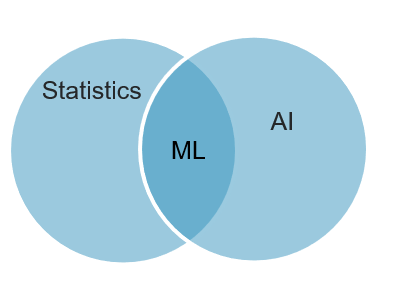
\includegraphics[width=0.95\textwidth]{pics/ml.png}
	\end{figure}
\end{columns}
\end{frame}

\begin{frame}
\frametitle{Lecture Overview}
\begin{block}{Chapters}
	\begin{enumerate}
		\item Basics and Linear Models
		\item Model Selection and Validation
		\item Trees
		\item Neural Nets
	\end{enumerate}
\end{block}

\begin{block}{Material}
	\url{https://github.com/mayer79/ml\_lecture}
\end{block}
\end{frame}

%=====================================================================
\section{Basics and Linear Models}
%=====================================================================

%=====================================================================
\subsection{Basics}
%=====================================================================

\begin{frame}
\frametitle{Before Modeling}
\begin{columns}
	\column{0.5\textwidth}
	\begin{itemize}
		\item Organization of data?
		\item Data types?
		\item Descriptive analysis
	\end{itemize}
	\begin{figure}
		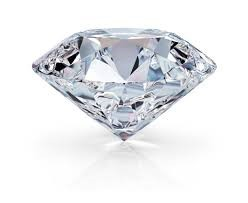
\includegraphics[width=0.6\textwidth]{pics/diamond.jpg}
	\end{figure}
	\column{0.5\textwidth}
	\begin{block}{Structure of diamonds data}
		\begin{figure}
			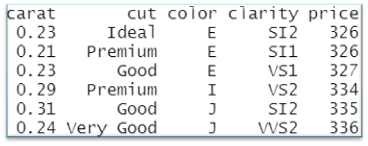
\includegraphics[width=0.95\textwidth]{pics/data_structure.png}
		\end{figure}
	\end{block}

	\begin{example}
	\end{example}
\end{columns}
\end{frame}

\begin{frame}
\frametitle{Statistical Models}
\begin{block}{Setting}
	\begin{itemize}
		\item Approximate \alert{response variable} $Y$ by function of \alert{covariates} $X_1,\dots,X_m$
		$$
			Y \approx f(X_1,\dots,X_m)
		$$
		\item Estimate unknown $f$ from data by $\hat f$.
		\item Use $\hat f$ for prediction and to investigate relationships.
		\item Postulate model equation
		$$
			\E(Y) = f(X_1, \dots, X_m)
		$$
		(we are often interested in means).
		\end{itemize}
	\end{block}
	
	\begin{block}{Remark}
	Other terms for response and covariates?
	\end{block}
\end{frame}

%=====================================================================
\subsection{Linear Regression}
%=====================================================================

\begin{frame}
\frametitle{Linear Regression}
\begin{itemize}
	\item Postulate 
	$$
		\E(Y) = f(X_1, \dots, X_m)=\beta_0 + \beta_1 X_1 + \dots + \beta_m X_m
	$$
	\item Interpretation of coefficients $\beta_j$? Ceteris Paribus!
	\item Optimal $\hat \beta_j$? Minimize sum of squared errors/residuals
	$$
		\sum_{i = 1}^n (\underbrace{y_i - \hat y_i}_{\text{\alert{Residual}}})^2 
	$$
	\item $\hat y = f(\dots)$ are \alert{predictions}
\end{itemize}

\begin{example}
	Simple linear regression 
	$$
		\E(Y)=\alpha = \beta X
	$$
\end{example}
\end{frame}

\begin{frame}
\frametitle{Aspects of Model Quality}
\begin{columns}[onlytextwidth]
	\column{0.5\textwidth}
	\begin{block}{Predictive performance}
		\begin{itemize}
			\item Absolute performance
				\begin{itemize}
					\item $\text{\alert{MSE}} = \frac{1}{n}\sum_{i = 1}^n (y_i - \hat y_i)^2$
					\item Root-MSE (\alert{RMSE})
					\item Loss and objective functions	
				\end{itemize}
			\item Relative performance
				\begin{itemize}
					\item \alert{R-squared}
				\end{itemize}
		\end{itemize}
	\end{block}	

	\column{0.5\textwidth}
	\begin{block}{Validity of assumptions}
		\begin{itemize}
			\item Model equation is correct
			\item {\em Normal} linear model
			 \begin{align*}
				 Y &= f(\dots) + \varepsilon \\
				 \varepsilon &\sim N(0, \sigma^2)
			 \end{align*}
		\end{itemize}
	\end{block}
\end{columns}
\begin{center}
	\begin{example}
	\end{example}
\end{center}
\end{frame}

\begin{frame}
\frametitle{Typical Problems}
\begin{itemize}
	\item Missing values
	
	\vfill
	
	\item Outliers
	
	\vfill
	
	\item Overfitting
	
	\vfill 
	
	\item Collinearity
\end{itemize}
\end{frame}

\begin{frame}
\frametitle{Categorical Covariates}
\begin{columns}
	\column{0.3\textwidth}
	\begin{itemize}
		\item One-Hot-Encoding
		\item Dummy coding
		\item Integer encoding
		\item Interpretation?
	\end{itemize}
	\vspace{1cm}
	\begin{example}
	\end{example}
	\column{0.65\textwidth}
	\begin{block}{Example of One-Hot-Encoding}
		\begin{figure}
			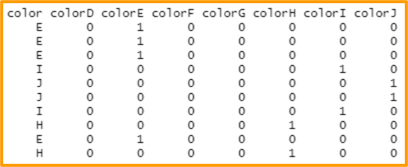
\includegraphics[width=0.95\textwidth]{pics/dummy.png}
		\end{figure}
	\end{block}
	\end{columns}
\end{frame}

\begin{frame}
\frametitle{Linear Regression is Flexible}
\begin{enumerate}
	\item Non-linear terms
	\item Interactions
	\item Transformations like logarithms
\end{enumerate}

\vfill

\begin{block}{These elements are essential but tricky!}
\end{block}
\end{frame}

\begin{frame}
\frametitle{Non-Linear Terms}
\begin{columns}
	\column{0.45\textwidth}
	\begin{block}{How to deal with non-linear associations to $Y$?}
		
		$\rightarrow$ use more parameters
	\begin{enumerate}
		\item Polynomial terms
		\begin{itemize}
			\item E.g., cubic regression
			$$
				\E(Y) = \beta_0 + \beta_1 x + \beta_2 x^2 + \beta_3 x^3
			$$
			\item Don't extrapolate!
		\end{itemize}
		\item Regression splines
	\end{enumerate}
	\end{block}
	
	\column{0.45\textwidth}
	\begin{block}{Example: Diamonds}
		Use systematic predictions
		\begin{figure}
			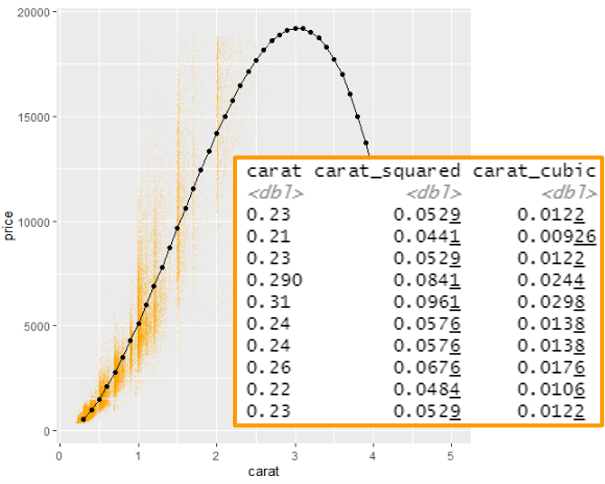
\includegraphics[width=0.95\textwidth]{pics/nonlinear.png}
		\end{figure}
	\end{block}
\end{columns}
\end{frame}

\begin{frame}
\frametitle{Interactions}
\begin{columns}
	\column{0.5\textwidth}
	\begin{itemize}
		\item Additivity of effects not always realistic
		$$
			\E(Y) = \beta + \beta_1 X_1 + \dots + \beta_m X_m
		$$
		\item Adding interaction terms brings necessary flexibility $\rightarrow$ more parameters
		\item Interaction between features $X$ and $Z$
		\begin{itemize}
			\item For categorical $Z$, effects of $X$ are calculated by level of $Z$
			\item Like separate models per level of $Z$
		\end{itemize}
	\end{itemize}
	
	\column{0.45\textwidth}
	\begin{block}{Example: Diamonds}
		\begin{figure}
			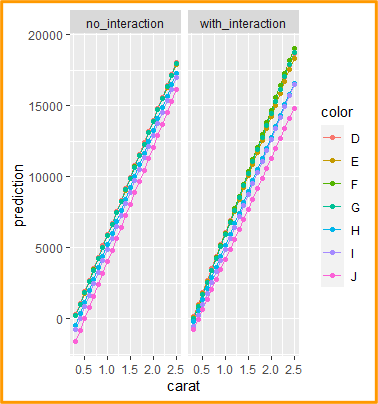
\includegraphics[width=0.95\textwidth]{pics/interactions.png}
		\end{figure}
	\end{block}
\end{columns}
\end{frame}

\begin{frame}
\frametitle{Transformations of Covariates}
\begin{block}{Examples}
	\begin{itemize}
		\item Dummy variables for categoricals
		\item Decorrelation
		\item Logarithms against outliers
	\end{itemize}
\end{block}

\vfill

Effects are interpreted for transformed covariates
\end{frame}

\begin{frame}
\frametitle{Logarithmic Covariates}
\begin{itemize}
	\item $\E(Y) = \alpha + \beta\log(X)$
	\item Properties of logarithm allow interpretation \alert{for original covariate}
	\item ``A 1\% increase in $X$ leads to an increase in $\E(Y)$ of about $\beta/100$''
	
	($\rightarrow$ lecture notes)
	
	\vfill
	
	\begin{example}
	\end{example}
\end{itemize}
\end{frame}

\begin{frame}
\frametitle{Logarithmic Responses}
What would happen for logarithmic response?
\begin{align*}
\E(\log(Y)) &= \alpha + \beta X \\
\implies \log(\E(Y)) &= \alpha + \beta X?
\end{align*}
The implication is wrong (why?) $\rightarrow$ biased predictions and motivation for GLMs

\begin{itemize}
	\item ``A one-point increase in $X$ is associated with a relative increase in $\E(Y)$ of $100\%(e^\beta - 1)\approx 100\% \beta$''
	$\rightarrow$ lecture notes
	\item Relative effects / multiplicative model
\end{itemize}

\begin{exampleblock}{Examples}
	\begin{itemize}
		\item Logarithmic response
		\item Response and covariate with log
	\end{itemize}
\end{exampleblock}
\end{frame}

\begin{frame}
\frametitle{Example: Realistic Model for Diamond Prices}
\begin{columns}
	\column{0.55\textwidth}
	\begin{itemize}
		\item Response: log(price)
		\item Covariates: log(carat), color, cut and clarity
	\end{itemize}
	\column{0.35\textwidth}
	\begin{figure}
		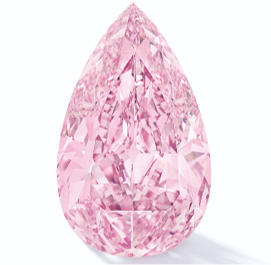
\includegraphics[width=0.7\textwidth]{pics/dia2.png}
	\end{figure}
\end{columns}
\end{frame}

\begin{frame}
\frametitle{Exercise on Linear Regression}
\begin{columns}
	\column{0.55\textwidth}
	\begin{itemize}
		\item Run last model without any logarithm
		\item Interpret the results
		\item Does model make sense from practical perspective?
	\end{itemize}
	\column{0.35\textwidth}
	\begin{figure}
		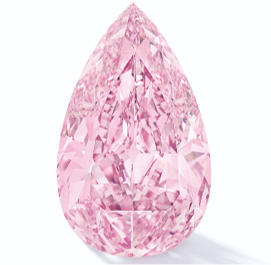
\includegraphics[width=0.7\textwidth]{pics/dia2.png}
	\end{figure}
\end{columns}
\end{frame}

%=====================================================================
\subsection{Generalized Linear Models}
%=====================================================================

\begin{frame}
\frametitle{Example: Realistic Model for Diamond Prices}
\begin{itemize}
	\item 
	\item
\end{itemize}
\end{frame}

%=====================================================================
\end{document}
%=====================================================================